\section{Zielsetzung}
    In diesem Versuch wird die Ablenkung von Elektronen in einem elektrischen, sowie in einem magnetischen Feld untersucht.

\section{Theorie}
\label{sec:Theorie}
    \subsection{Erzeugug eines Elektronenstrahls in einer Kathodenstrahlröhre}
    In diesem Versuch wird eine Kathodenstrahlröhre verwendet wie sie in \autoref{fig:wehnelt} schematisch dargestellt ist.
    Im Wesentlichen besteht diese Kathodenstrahlröhre aus drei Komponenten: einer sogenannten Elektronenkanone, einem Ablenksystem und einem 
    Nachweissystem. In der Elektronenkanone werden Elektronen mittels Glühemission aus der Kathode, welche aus einem Material mit 
    geringer Austrittsarbeit besteht, gelöst. Die Intensität des Strahls kann dabei über den Wehneltzylinder geregelt werden, welcher die
    Kathode umgibt. Davor befindet sich eine Elektrode mit im Vergleich zur Kathode hohem Potential, welche die Elektronen beschleunigt.
    Hinter der Beschleunigungselektrode befinden sich weitere Elektroden, welche den Elektronenstrahl fokussieren. Darauf folgend befindet sich das 
    Ablenksystem, welches aus zwei Plattenpaaren, je ein Paar für je eine abzulenkende Raumrichtung, besteht. Durch Anlegen einer Spannug an die
    Platten lenkt das enstehende elektrische Feld die Elektronen ab. Dies ist im Nachweissystem sichtbar, welches hier ein Leuchtschirm ist.
    Wenn die Elektronen auf den Schirm fallen, regen sie sogenannte Aktivatorzentren an, welche im angeregten Zustand Lichtquanten emittieren.
    Auf diese Weise kann die Ablenkung sichtbar gemacht und ausgemessen werden.
    Zu Erwähnen sei noch, dass die Kathodenstrahlröhre bis auf einen geringen Restdruck evakuiert ist, um Wechselwirkungen der Elektronen mit 
    den Molekülen der Luft auszuschließen und damit das Ergebnis nicht zu verfälschen.
    \begin{figure}
        \centering
        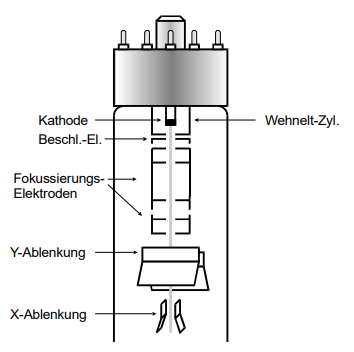
\includegraphics[width=0.6\textwidth]{content/wehnelt.png}
        \caption{Aufbau des Kathodenstrahlrohrs \cite{V501-und-V502}.}
        \label{fig:wehnelt}
    \end{figure}

\subsection{Ablenkung des Elektronenstrahls in einem elektrischen Feld}
    Wenn Elektronen ein elektrisches Feld passieren, wirkt eine Kraft $F$ auf sie, was als Ablenkung von der ursprünglichen Bahn auf dem 
    Detektorschirm zu sehen ist. Zur Veranschaulichung der Zusammenhänge wird sich hier auf \autoref{fig:ablenk} bezogen. Solange der 
    Abstand $d$ zwischen den Platten wesentlich geringer als deren Länge $p$ ist, kann das elektrische Feld näherungsweise als
    homogen angenommen werden. Die Kraft die auf ein einzelnes Elektron wirkt ist dann
    \begin{equation}
    \label{eqn:e_kraft}
        \lvert \vec{F} \rvert = \lvert e_0 \vec{E} \rvert = e_0 \frac{U_{\symup{d}}}{d},
    \end{equation}    
    wobei $e_0$ die Elementarladung, $\vec{E}$ das homogene elektrische Feld und $U_{\symup{d}}$ die angelegte Ablenkspannung ist.
    Darüberhinaus lässt sich die Verschiebung $D$ des Elektronenstrahls auf dem Leuchtschirm zu
    \begin{equation}
    \label{eqn:e_verschiebung}
        D = \frac{p}{2 d} L \frac{U_{\symup{d}}}{U_{\symup{B}}}
    \end{equation}
    bestimmen. Hierbei ist $L$ der Abstand zwischen Kathode und Detektorschirm und $U_{\symup{B}}$ die angelegte Beschleunigungsspannung.
    \begin{figure}
        \centering
        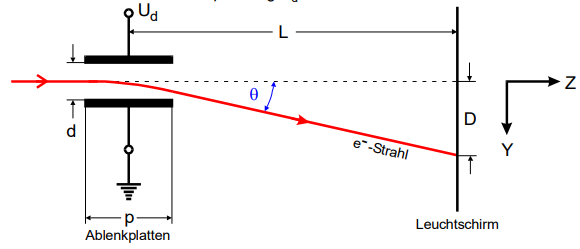
\includegraphics[width=0.7\textwidth]{content/eablenk.png}
        \caption{Schematische Darstellung der Strahlablenkung im Kathodenstrahlrohr \cite{V501-und-V502}.}
        \label{fig:ablenk}
    \end{figure}
\subsection{Kathodenstrahl-Oszillograph}
\label{sec:oszillo}
    Das zuvor beschriebene Kathodenstrahlrohr kann so umgebaut werden, dass es zur Darstellung der Zeitabhängigkeit von Wechselspannungen
    genutzt werden kann. Dazu wird eine Sägezahnspannung an die Platten für die horizontale Ablenkung angeschlossen.
    An das andere Plattenpaar wird die Spannung angeschlossen, welche es zu untersuchen gilt.
    Durch korrekte Einstellung des Frequenzverhältnisses der beiden angelegten Spannungen ist es möglich den zeitlichen Verlauf der 
    angelegten Wechselspannung auf dem Detektorschirm darzustellen. Dazu muss gelten:
    \begin{equation}
    \label{eqn:frequenz}
         n \nu_{\symup{Sä}} = m \nu_{\symup{We}}; \, n,m \in \symbb{N}.
    \end{equation}     
    Hierbei bezeichnet $\nu_{\symup{Sä}}$ die Frequenz der Sägezahnspannung und $\nu_{\symup{We}}$ die Frequenz der zu untersuchenden 
    Wechselspannung.
\subsection{Ablenkung des Elektronenstrahls in einem homogenen Magnetfeld}
    Ein annähernd homogenes Magnetfeld kann durch ein Helmholtzspulenpaar erzeugt werden. Dieses erechnet sich in der Mitte des Spulenpaares 
    über 
    \begin{equation}
    \label{eqn:helmholtz}
        B = \mu_0 \frac{8}{\sqrt{125}} \frac{N I}{R},
    \end{equation}
    wobei $N$ die Windungsanzahl, $I$ die Stromstärke, $R$ der Spulenradius und $\mu_0$ die magnetische Feldkonstante ist.
    In einem homogenen Magnetfeld wirkt die sogenannte Lorentzkraft
    \begin{equation}
    \label{eqn:lorentz}
        \vec{F_{\symup{L}}} = q \cdot \vec{v} \times \vec{B}
    \end{equation}    
    auf bewegte Ladungen. Dabei ist $q = e_0$ die Ladung eines Elektrons, $\vec{v}$ die Geschwindigkeit des Elektrons und $\vec{B}$ die  
    Stärke des angelegten Magnetfeldes. Da die potentielle Energie der Elektronen konstant ist, gilt nach der Energieerhaltung, dass 
    $\lvert \vec{v} \rvert = v_0$ ebenfalls konstant sein muss. Durch Gleichsetzen der Lorentzkraft mit der Zentrifugalkraft ergibt sich der 
    Krümmungsradius der abgelenkten Bahn zu
    \begin{equation}
    \label{eqn:kruemmungsradius}
        r = \frac{m_0 v_0}{e_0 B},
    \end{equation}
    wobei $m_0$ die Masse eines Elektrons ist. Bei Anlegung eines konstanten Magnetfeldes ist der gesamte rechte Term der Gleichung konstant.
    Daraus folgt, dass sich das Elektron auf einer Kreisbahn bewegt.

\subsection{Spezifische Elektronenladung}
    Für den Krümmungsradius $r$ kann mittels geometrischer Überlegungen, dargestellt in \autoref{fig:zusammenhang}, ein 
    Zusammenhang zur Länge $L$ des Kathodenstrahlrohrs und der Ablenkung $D$ auf dem Detektorschirm hergestellt werden.
    Dazu wird außerdem der Energiesatz
    \begin{equation}
    \label{eqn:energiesatz}
        v_0 = \sqrt{2 \frac{U_{\symup{B}}} e_0} {m_0}
    \end{equation}
    verwendet. Es folgt:
    \begin{equation}
    \label{eqn:zusammenhang}
        r = \frac{L^2 + D^2}{2D},    
    \end{equation}     
    womit sich für die spezifische Ladung die Gleichung
    \begin{equation}
    \label{eqn:spezifisch}
        \frac{e_0}{m_0} = \frac{8 U_{\symup{B}} D^2}{(L^2 + D^2)B^2}
    \end{equation}
    ergibt.    
    \begin{figure}
        \centering
        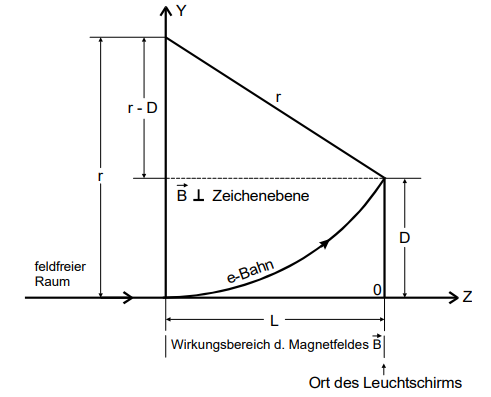
\includegraphics[width=0.7\textwidth]{content/zusammenhang.png}
        \caption{Skizze zur Bestimmung der geometrischen Beziehungen zwischen $L$, $D$ und $r$ \cite{V501-und-V502}.}
        \label{fig:zusammenhang}
    \end{figure}